\documentclass{article}
\usepackage{pgfplots}
\pgfplotsset{width=9cm,compat=1.5}
\pgfplotsset{every axis legend/.append style={ at={(0.9,0.2)},anchor=north east}} 
\begin{document}

%Ram time
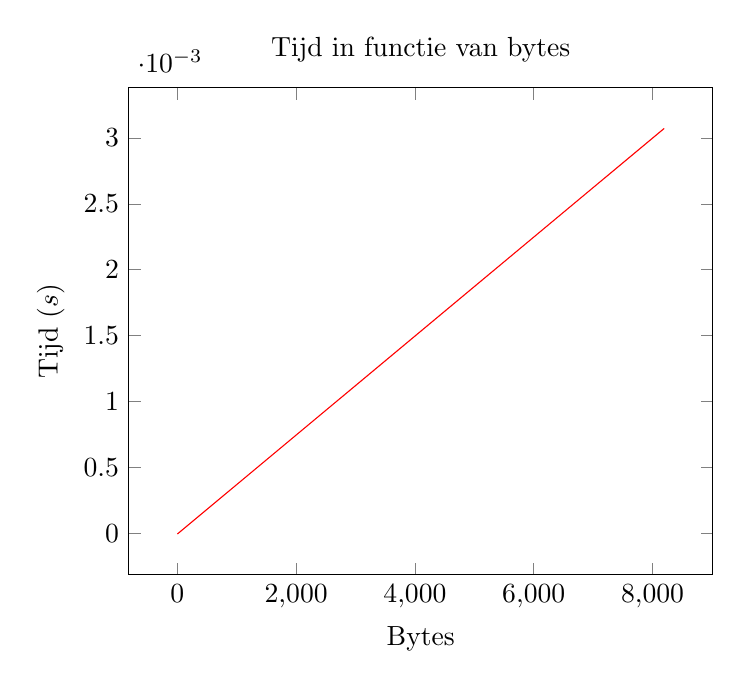
\begin{tikzpicture}
\begin{axis}[
title=Tijd in functie van bytes,
xlabel={Bytes},
ylabel={Tijd $(s)$}
]
\addplot[
red,
domain=0:8196,
samples=201,
]
{3.752E-7 *x -3.773E-6};
\end{axis}
\end{tikzpicture}

%Ram energy
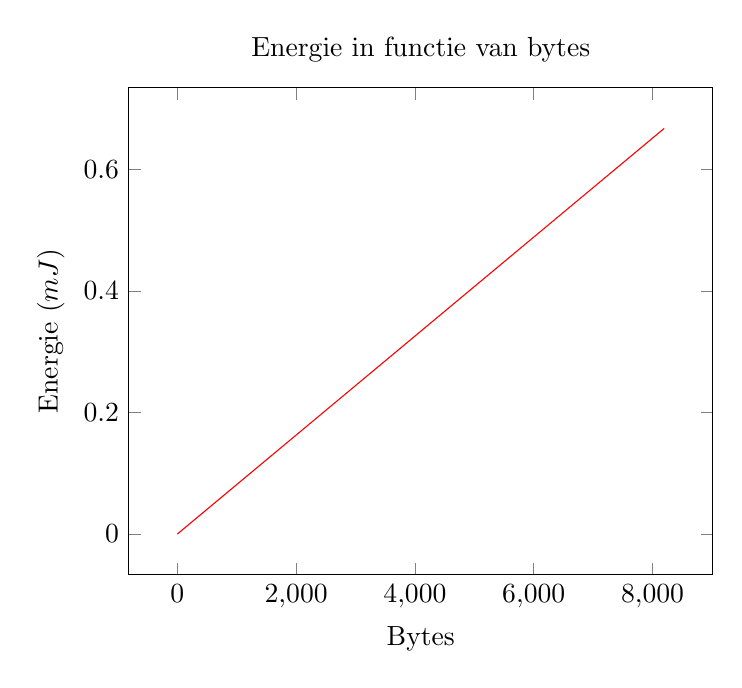
\begin{tikzpicture}
\begin{axis}[
title=Energie in functie van bytes,
xlabel={Bytes},
ylabel={Energie $(mJ)$}
]
\addplot[
red,
domain=0:8196,
samples=201,
]
{8.144E-5 * x };
\end{axis}
\end{tikzpicture}

%CPU engergie
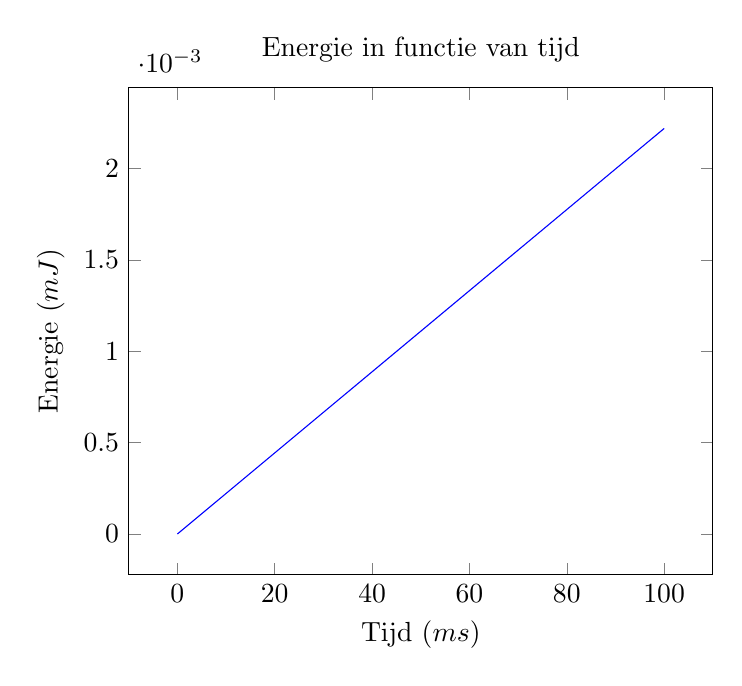
\begin{tikzpicture}
\begin{axis}[
title=Energie in functie van tijd,
xlabel={Tijd $(ms)$},
ylabel={Energie $(mJ)$}
]
\addplot[
blue,
domain=0:100,
samples=201,
]
{0.0037 * x *1E-3 *6};

\end{axis}

\end{tikzpicture}

%Energie idleness + energie ram
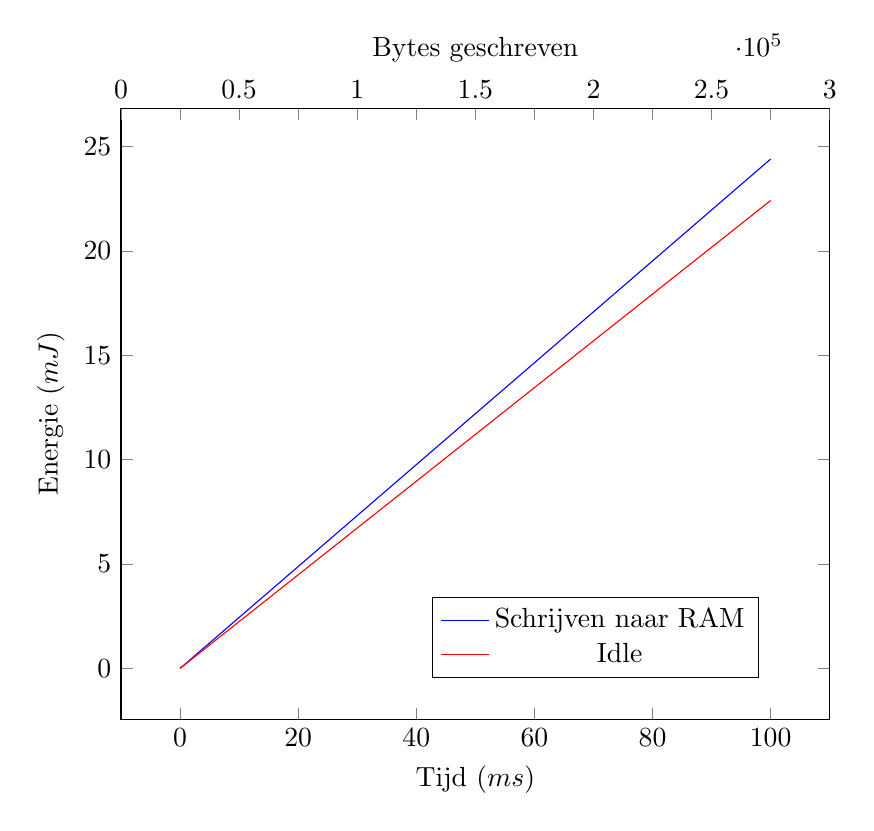
\begin{tikzpicture}
\begin{axis}[
scale only axis,
xlabel={Tijd $(ms)$},
ylabel={Energie $(mJ)$}
]
\addplot[
blue,
domain=0:100,
samples=201,
]
{x/0.000333638186177248 * 8.144E-5 };
\addplot[
red,
domain=0:100,
samples=201,
]
{x * 0.224222886125917 };
\legend{Schrijven naar RAM,Idle,$l_3$}
\end{axis}
\begin{axis}[
scale only axis,
ymin=0,ymax=300000,
xmin=0,xmax=300000,
xlabel={Bytes geschreven},
axis x line*=top,
hide y axis,
]
\end{axis}
\end{tikzpicture}


%Energie idleness + energie ram
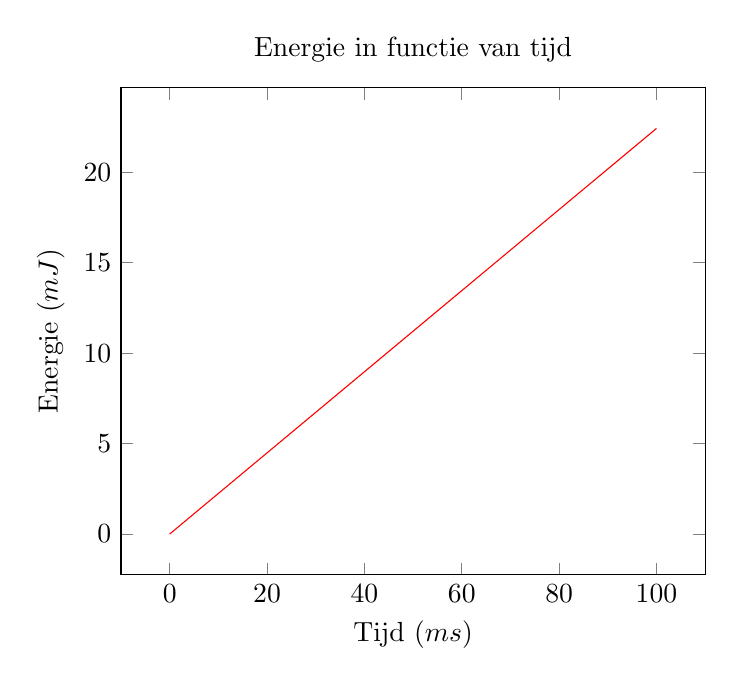
\begin{tikzpicture}
\begin{axis}[
title=Energie in functie van tijd,
xlabel={Tijd $(ms)$},
ylabel={Energie $(mJ)$}
]
\addplot[
red,
domain=0:100,
samples=201,
]
{x * 0.224222886125917 };


\end{axis}
\end{tikzpicture}





\begin{tikzpicture}
\begin{axis}[
xlabel={$x$},
ylabel={$y$},
]
\addplot[blue] table {CPU-naive.tsv};
\end{axis}
\end{tikzpicture}	


% Idle
\begin{tikzpicture}
\begin{axis}[
title=Energie in functie van tijd,
xmin=0.5,xmax=2,
xlabel={Tijd $(ms)$},
ylabel={Energie $(mJ)$},
]
\addplot[blue] table {cpu1.dat};
\addplot[red] table {cpu2.dat};
\addplot[green] table {cpu3.dat};
\addplot[yellow] table {cpu4.dat};
\addplot[gray] table {cpu5.dat};
\end{axis}
\end{tikzpicture}	
\end{document}